\chapter{Testing and Application}

This chapter contains an overview of the testing performed for the development of \stops\ (\autoref{sec:test_stops}) and the checking of the replaced wavelength solutions (\autoref{sec:test_wav}), as well as the application of \stops\ on observations (\autoref{sec:results_unpub}) and its application in publications (\autoref{sec:results_pub}).

% MARK: Test STOPS
\section[Testing \textsc{stops}]{Testing \stops} \label{sec:test_stops}

% No \polsalt\ tests or tests on pre-reduced \gls{FITS} files. (Trusted accurate)
% General discussion of testing (I.E. not this test was done specifically this source, more along the lines of these tests were done to check this issue, seen here using this source for example.)
The main challenge faced when developing \stops\ was ensuring that the software was compatible with both the \polsalt\ and \iraf\ file structures. As development is an iterative process, \stops\ was continually checked to ensure compatibility such that the varying \stops\ method inputs were correctly parsed, and that their outputs were parsable by the relevant \iraf\ tasks or \polsalt\ methods.

To this end, observations which were verified to have been accurately reduced were duplicated for testing purposes, allowing for continual checks of the \stops\ pipeline to be made during the development process. As the \stops\ \texttt{split} and \texttt{join} methods are designed to convert between the \polsalt\ and \iraf\ file structures, greater emphasis was made to ensure that the output of both methods provided accurate and consistent results.

% % Why the pipeline is better
% The rigorous error handling in \stops\ ensures that the user is informed of any issues that arise during the reduction process. This is particularly important as \stops\ was developed to enable a faster reduction process compared to that of pure \iraf\ or \polsalt.

% Reduction specific tests refer to tests performed to ensure no errant effects are introduced during the reduction process. These tests were designed to validate the accuracy and reliability of the \stops\ pipeline in producing scientifically accurate results.

% MARK: STOPS split tests
\subsection{Testing the \texttt{split} Method} \label{subsec:test_split}

The \stops\ \texttt{split} method requires any \polsalt\ pre-reduced (`mxgbp'- prefixed) \gls{FITS} files as input and outputs \iraf\ compatible (`(arc|beam)(O|E)'- prefixed) \gls{FITS} file structures. As no `split' \gls{FITS} files are created during pure \polsalt\ reductions, the \stops\ \texttt{split} method was tested by comparing the pre-reduced \polsalt\ files to the \texttt{split} method's output files, ensuring the correct structure and data integrity of the files handed off to \iraf.

% \newcommand\mc[1]{\multicolumn{1}{c|}{#1}} % handy shortcut macro

\begin{table}[t]

    \centering

    \caption{A comparison of the contents of a \polsalt\ pre-reduced \gls{FITS} file to the \stops\ \texttt{split} $O$- and $E$-beam \gls{FITS} files. Table created using the `\texttt{Astropy}' \texttt{fitsinfo} \gls{CLI} tool.}
    \label{table:split_info}

    \begin{tabular}{lcccccc}
        \toprule
        Filename &
        No. &
        Name &
        Type &
        Cards &
        Dimensions &
        Format \\
        \midrule
        \polsalt % mxgbpP201703280054.fits
        & $0$ & \gls{PRIMARY} & PrimaryHDU & $161$   & -                & -       \\
        & $1$ & \gls{SCI}     & ImageHDU   & $19$    & ($3199$, $1028$) & float32 \\
        & $2$ & \gls{VAR}     & ImageHDU   & $8$     & ($3199$, $1028$) & float32 \\
        & $3$ & \gls{BPM}     & ImageHDU   & $8$     & ($3199$, $1028$) & uint8   \\
        \stops\ \texttt{split} `$O$' % beamo0054.fits
        & $0$ & \gls{PRIMARY} & PrimaryHDU & $162$   & ($3199$, $474$)  & float32 \\
        \stops\ \texttt{split} `$E$' % beame0054.fits
        & $0$ & \gls{PRIMARY} & PrimaryHDU & $162$   & ($3199$, $474$)  & float32 \\ \bottomrule
    \end{tabular}

\end{table}


\autoref{table:split_info} shows the \gls{FITS} file information for the files before and after splitting. The split \gls{FITS} files contain the split \gls{SCI} extension data and the \gls{PRIMARY} header from the pre-reduced files, with any Header or Data differences mentioned below.

The header is left mostly untouched, and is only updated to represent the new data type and shape:
the `BITPIX' value is updated, from $8$ to $-32$, and the `NAXIS' value is updated, from $0$ to $2$;
the `NAXIS1' and `NAXIS2' keywords are added, and their values are set to the new split \gls{SCI} data shape;
and the `EXTEND' keyword is removed.%
\footnote{The `EXTEND' keyword indicates that the \gls{FITS} file contains multiple extensions while the `NAXIS1' and `NAXIS2' keywords indicate the shape and size of the data stored in the relevant extension.}
This accounts for the discrepancy in the `Cards' between the \polsalt\ and \stops\ file header entries in \autoref{table:split_info}.

\begin{figure}
    \centering
    \begin{subfigure}[b]{\textwidth}
        \centering
        
\includegraphics[width=\textwidth]{4_diff_O.pdf}
        \caption{The difference in the \gls{SCI} extensions, for the `O' polarization beam.}
        \label{subfig:diff_split_O}
    \end{subfigure}
    \hfill
    \begin{subfigure}[b]{\textwidth}
        \centering
        
\includegraphics[width=\textwidth]{4_diff_E.pdf}
        \caption{The difference in the \gls{SCI} extensions, for the `E' polarization beam.}
        \label{subfig:diff_split_E}
    \end{subfigure}
    \caption{The difference between the \polsalt\ pre-reduced (`mxgbp'- prefixed) \gls{FITS} files and the \stops\ `split' (`(arc|beam)(O|E)'- prefixed) files. Figures created using both the \polsalt\ \texttt{Raw image reduction} and \stops\ \texttt{split} method outputs.}
    \label{fig:split_diff}
\end{figure}

\autoref{fig:split_diff} shows that the \polsalt\ \gls{SCI} data is unmodified when copying the data to the \stops\ \gls{FITS} file, but only includes half of the data, for the relevant $O$- or $E$-polarization beam, \autoref{subfig:diff_split_O} and \autoref{subfig:diff_split_E}, respectively, with a cropping which defaults to $40$~pixels (see \autoref{subsec:stops_split}), introduced to the top- and bottom-most rows of the \polsalt\ data. This accounts for the discrepancy in the `Dimensions' between the \polsalt\ and \stops\ files in \autoref{table:split_info}.

This output file structure was chosen for \iraf\ compatibility, and was tested over multiple grating and articulation angles, as well as with various data sets to ensure that the \texttt{split} method was robust and reliable.

% MARK: STOPS join tests
\subsection{Testing the \texttt{join} Method} \label{subsec:test_join}

The \texttt{join} method requires both an \iraf\ database with wavelength solutions (or a custom wavelength solution) for both polarimetric beams and the \polsalt\ pre-reduced files as input and outputs \polsalt\ \texttt{spectra extraction} compatible (`wmxgbp'- prefixed) \gls{FITS} file structures. Ensuring that the output format was correct was paramount as the \polsalt\ \texttt{spectra extraction} method is unable to process the files otherwise, thus halting the reduction process. Thankfully, the \texttt{join} method output could be compared to the \polsalt\ \texttt{wavelength calibration} method output files, ensuring that any changes introduced by the \stops\ pipeline were well characterized.

\begin{table}[t]

    \centering

    \caption{A comparison of the \polsalt\ wavelength calibrated \gls{FITS} file to the (\iraf\ wavelength calibrated) \stops\ \texttt{join} \gls{FITS} file. Table created using the \texttt{Astropy} \texttt{fitsinfo} \gls{CLI} tool.}
    \label{table:join_info}

    \begin{tabular}{lcccccc}
        \toprule
        Filename &
        Ext. No. &
        Name &
        Type &
        Cards &
        Dimensions &
        Format \\
        \midrule
        \polsalt % wmxgbpP201703280054.fits
        & $0$ & \gls{PRIMARY} & Primary\gls{HDU} & $161$ & -             & -       \\
        & $1$ & \gls{SCI} & Image\gls{HDU} & $21$ & ($3199$, $514$, $2$) & float32 \\
        & $2$ & \gls{VAR} & Image\gls{HDU} & $10$ & ($3199$, $514$, $2$) & float32 \\
        & $3$ & \gls{BPM} & Image\gls{HDU} & $10$ & ($3199$, $514$, $2$) & uint8   \\
        & $4$ & \gls{WAV} & Image\gls{HDU} & $21$ & ($3199$, $514$, $2$) & float32 \\
        \stops\ \texttt{join} % wmxgbpP201703280054.fits
        & $0$ & \gls{PRIMARY} & Primary\gls{HDU} & $161$ & -             & -       \\
        & $1$ & \gls{SCI} & Image\gls{HDU} & $21$ & ($3199$, $474$, $2$) & float32 \\
        & $2$ & \gls{VAR} & Image\gls{HDU} & $10$ & ($3199$, $474$, $2$) & float32 \\
        & $3$ & \gls{BPM} & Image\gls{HDU} & $10$ & ($3199$, $474$, $2$) & uint8   \\
        & $4$ & \gls{WAV} & Image\gls{HDU} & $21$ & ($3199$, $474$, $2$) & float32 \\
        \bottomrule
    \end{tabular}

\end{table}


\autoref{table:join_info} shows the \gls{FITS} file information for both the \polsalt\ and \stops\ wavelength calibrated files. Other than the `Dimensions' of each `ImageHDU' extension,%
\footnote{The `Dimensions' differ due to the before mentioned cropping of the top- and bottom-most rows of the data.}
the \gls{FITS} files are identical in structure.

Although the `Cards' count is the same, minor differences across the headers are present. The `HISTORY' keyword, which contains the \polsalt\ `CRCLEAN' parameters and which default to `upper= 4.0, lower= 1.5, sigmaveto= 2.0', is left as `None' in the \stops\ file.%
\footnote{The \polsalt\ pipeline performs cosmic ray cleaning using a $10\sigma$ spike to cull cosmic rays. See the \polsalt\ \protect\href{https://github.com/saltastro/polsalt/blob/master/polsalt/specpolwavmap.py\#L132}{source code} for more information.}
Although \stops\ performs cosmic ray cleaning (see \autoref{subsec:stops_join}), the parameters are not stored in the header as \polsalt\ and \stops\ implement different methods for cosmic ray cleaning. Other minor differences such as the date-times stored in the `SAL-TLM' and `SMOSAIC' keywords may also differ as they contain the date-times relating to the completion of the \polsalt\ pre-reductions. This accounts for the differences in the `Cards' between the \polsalt\ and \stops\ file header entries in \autoref{table:join_info}.

\begin{figure}
    \centering
    \begin{subfigure}[b]{\textwidth}
        \centering
        
\includegraphics[width=\textwidth]{4_diff_SCI.pdf}
        \caption{The difference in the \gls{SCI} extensions.}
        \label{subfig:join_SCI}
    \end{subfigure}
    \hfill
    \begin{subfigure}[b]{\textwidth}
        \centering
        
\includegraphics[width=\textwidth]{4_diff_VAR.pdf}
        \caption{The difference in the \gls{VAR} extensions.}
        \label{subfig:join_VAR}
    \end{subfigure}
    \hfill
    \begin{subfigure}[b]{\textwidth}
        \centering
        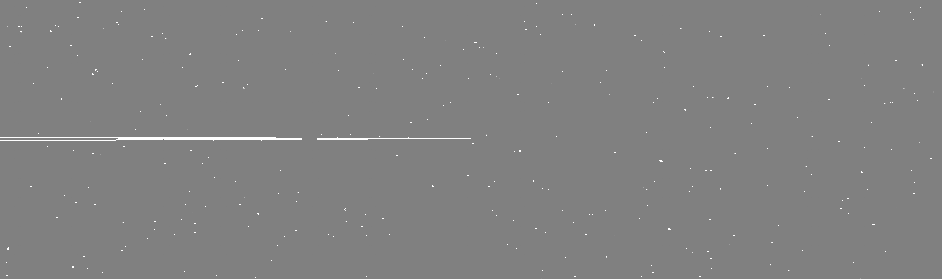
\includegraphics[width=\textwidth]{4_diff_BPM.pdf}
        \caption{The difference in the \gls{BPM} extensions.}
        \label{subfig:join_BPM}
    \end{subfigure}
    \hfill
    \begin{subfigure}[b]{\textwidth}
        \centering
        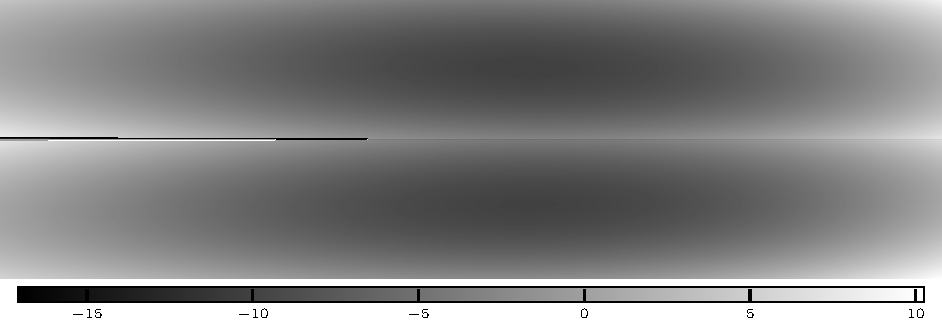
\includegraphics[width=\textwidth]{4_diff_WAV.pdf}
        \caption{The difference in the \gls{WAV} extensions.}
        \label{subfig:join_WAV}
    \end{subfigure}
    \caption{The difference of the \gls{FITS} file extensions between the \polsalt\ and \stops\ (`wmxgbp'- prefixed) wavelength calibrated files. Figures created using both the \polsalt\ and \stops versions of the \polsalt\ \texttt{spectral extraction} input.}
    \label{fig:join_in_out_diff}
\end{figure}

\autoref{fig:join_in_out_diff} shows the differences in the data between the \polsalt\ and \stops\ wavelength calibrated files. It can be seen that the \gls{VAR} extensions (\autoref{subfig:join_VAR}) are identical. The \gls{SCI} extensions (\autoref{subfig:join_SCI}) differ only in that the cosmic ray cleaning has been applied to the \stops\ data, whereas the \polsalt\ data applies a mask to the cosmic rays using the \gls{BPM} extension (\autoref{subfig:join_BPM}). The \gls{BPM} and \gls{WAV} extensions (\autoref{subfig:join_WAV}) are also masked to account for the valid wavelength calibrated region. The \gls{WAV} extensions contain the differing wavelength solutions and as such naturally differ. This accounts for the differences in the data between the \polsalt\ and \stops\ files.

Finally, the \stops\ \texttt{join} method was tested to ensure compatibility and correctness of the output data in comparison to \polsalt. This involved testing the \texttt{join} method with various data sets to ensure that the output files were accurate and consistent.

% MARK: Check Wav. Cal.'s
\section{Wavelength Solution Checks} \label{sec:test_wav}

% No \iraf\ tests or tests on \iraf\ \gls{FITS} files. (Trusted accurate)
The secondary challenge encountered when developing \stops\ was ensuring that the wavelength solutions parsed by \stops\ were unaffected by the pipeline and that they were similar to those created by \polsalt. This was achieved through the \texttt{correlate} and \texttt{skylines} methods, which were designed to validate the wavelength solutions produced by \iraf, but were later modified to parse both the \iraf\ and \polsalt\ wavelength solutions, allowing for further inspection of the two-dimensional wavelength solution.

Before the \polsalt\ wavelength calibrations were replaced with the \iraf\ wavelength calibrations, the accuracy of the new wavelength solutions needed to be validated. This was done both through the \iraf\ tasks, ensuring an accurate wavelength solution, and through the \stops\ \texttt{correlate} and \texttt{skylines} methods, allowing the integration of the wavelength solutions to be validated.

\todo{Add \gls{RMS} results (Table / Figures / Both?) from wavelength solution checks (\iraf\ \gls{RMS}, \polsalt\ \gls{RMS}) to quantify differences.}

\todo{Plot \iraf\ vs \polsalt\ \gls{RMS} for sources?}

% MARK: WAV Corr. Checks
\subsection{Cross Correlation Checks} \label{subsec:test_corr}

% O/E correlation checks to verify the consistency of the wavelength solutions.
The \texttt{correlate} method returns plots validating the wavelength solutions and so only has to accept the \polsalt\ \texttt{spectra extraction} (`ecwmxgbp'- prefixed) method output files as input.

\begin{figure}
    \centering
    \begin{subfigure}[b]{\textwidth}
        \centering
        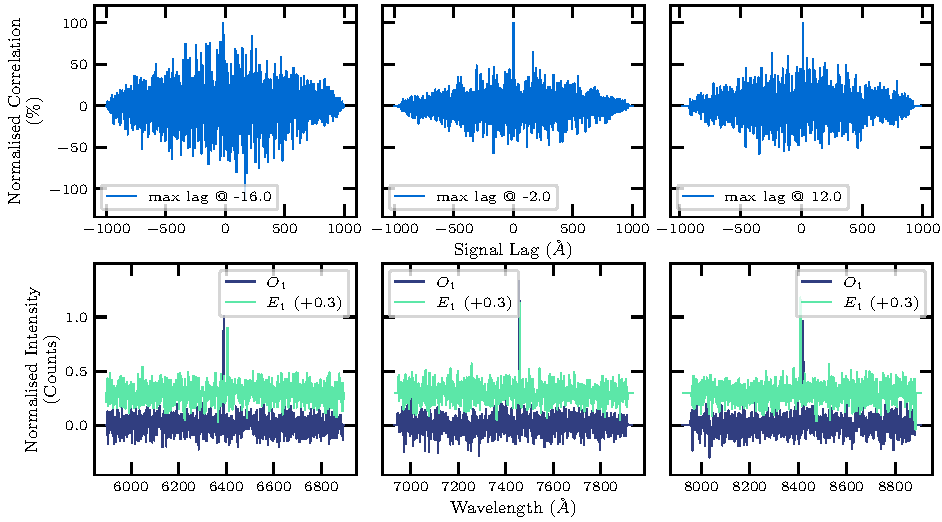
\includegraphics[width=\textwidth]{4_corr_test.pdf}
        \caption{fig1 caption}
        \label{subfig:fig1_label}
    \end{subfigure}
    \hfill
    \begin{subfigure}[b]{\textwidth}
        \centering
        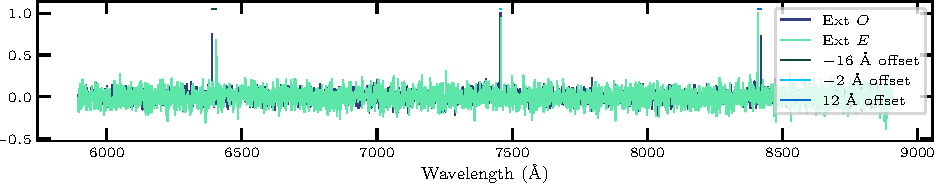
\includegraphics[width=\textwidth]{4_corr_spec.pdf}
        \caption{fig2 caption}
        \label{subfig:fig2_label}
    \end{subfigure}
    \caption{Overall caption}
    \label{fig:fig_caption}
\end{figure}

\todo{Show testing `correlate' functionality using `offset', comparisons of arcs, FSRQ's (few features) and BLLac's (many features).}

\todo{Insert figure(s) illustrating cross correlation accuracy.}

% MARK: WAV Sky. Checks
\subsection{Sky Line Checks} \label{subsec:test_sky}

% Full frame wavelength solution checks to ensure comprehensive calibration.
% Verifying the accuracy of the cross-correlation function against known standards.
The \texttt{skylines} method returns plots validating the wavelength solutions and so only has to accept either the \iraf\ \texttt{transform} task or \stops\ \texttt{join} method output files as input.

\todo{Compare skylines from \stops\ to `poor' \polsalt\ spectral extraction (I.E. spectral extraction with no trace in the `target' window and the `background' window on region with no skylines).}

\todo{Test `skylines' using known spectral sky lines / telluric lines.}

\todo{Insert figure illustrating skyline identification accuracy.}

% MARK: Application
\section[Application of \textsc{stops}]{Application of \stops}
% https://ui.adsabs.harvard.edu/search/fq=%7B!type%3Daqp%20v%3D%24fq_database%7D&fq_database=database%3Aastronomy&p_=0&q=%20author%3A%22Cooper%2C%20J.%22%20spectropolarimetry&sort=date%20desc%2C%20bibcode%20desc

\todo{1-2 paragraph intro mentioning both standards used for testing and (flaring blazar) science targets used. Mention results discussed for optical region, and briefly why (\gls{SALT}).}

% MARK: spec. pol. std.'s
\subsection{Spectropolarimetric Standards} \label{sec:results_unpub}

Testing included the use of spectropolarimetric standards, comprising four highly polarized and two non-polarized objects. \todo{VERIFY CORRECT}

\todo{Insert table listing the spectropolarimetric standards used, with their properties.}

\subsubsection{Source}

\todo{For each standard:}

\todo{Mention basic background information and a general discussion for source (A little more detail than included in paper).}

\todo{General reduction steps performed (not necessary to constantly repeat self). Highlight any differences in reduction steps compared to science targets.}

\todo{Insert figure(s) showing comparison plots of spectrum/polarization parameters from \polsalt\ and \stops (or leave out \polsalt\ and just show comparison to ($FORS1/2$) published results). Also short discussion (what the results can tell us and why it is useful). Focus on polarization results.}

\todo{Add a `see \ ref{reference}' to final paragraph and, if one of my papers, mention attached in appendix.}

% MARK: Science Targets
\subsection{Spectropolarimetric Science Targets} \label{sec:results_pub}

Tested using 3C 279, 4C+01.02, and preliminary testing data provided by David. \todo{VERIFY CORRECT}

% \begin{itemize}
%     \item Hester paper(s)
%     \item Joleen proceedings and work
%     \item My proceedings
% \end{itemize}
\todo{Insert table listing the spectropolarimetric targets used, with their properties.}

\subsubsection{Source}

\todo{For each published target:}

\todo{Mention basic background information and a general discussion for source (summary of paper + and necessary extra).}

\todo{General reduction steps performed (not necessary to constantly repeat self).}

\todo{Insert figure(s) showing comparison plots of spectrum/polarization parameters from \polsalt\ and \stops (or leave out \polsalt\ and just show published results). Also short discussion (what the results can tell us and why it is useful). Focus on polarization results.}
